\section{Appendix}
\label{sec:appendix}
\suppressfloats[t]  % no float above the Appendix heading on its own page

\subsection{Readouts and statistics}
\label{sec:app-readouts}

% Table A1: how bad endings start. Body generated by dramatis scripts/paper_tables.py (make tables).
\begin{table}[tbp]
  \centering
  \small
  \caption{
    \textbf{How bad endings start.}
    In the corpus: every bad ending of the four performed acts.
    Model-generated: using pretrained $z=0$ models, 1M--100M, 3 seeds pooled, villain names, restricted to endings judged as ``bad.''
    Prewritten: the 64 bad endings (4 acts, 16 items per act).
  }
  \label{tab:starts}
  \begin{tabular}{lrrrr}
\toprule
 & \multicolumn{3}{c}{The ending starts with} & \\
\cmidrule(lr){2-4}
 & the child's name & ``While'' or ``When'' & a quote & $n$ \\
\midrule
\multicolumn{5}{@{}l}{\emph{In the corpus, as written}} \\
Steal & 18\% & 82\% & 0\% & 559{,}061 \\
Cheat & 59\% & 40\% & 0\% & 560{,}648 \\
Tease & 0\% & 0\% & 100\% & 559{,}839 \\
Lie & 0\% & 0\% & 100\% & 560{,}452 \\
\midrule
\multicolumn{5}{@{}l}{\emph{Model-generated endings, villain names}} \\
Steal & 9\% & 91\% & 0\% & 953 \\
Cheat & 59\% & 41\% & 0\% & 924 \\
Tease & 0\% & 0\% & 100\% & 922 \\
Lie & 0\% & 0\% & 100\% & 959 \\
\midrule
Prewritten endings, all four acts & 100\% & 0\% & 0\% & 64 \\
\bottomrule
\end{tabular}

\end{table}

% Table A2: the two readouts compared. Body generated by dramatis scripts/paper_tables.py (make tables).
\begin{table}[tbp]
  \centering
  \small
  \caption{
    \textbf{Comparing prewritten and model-generated readouts.}
    ``Ben steals'' at 10M. Mean with 95\% CI over 8 seeds.
    At $z=1$, the prewritten readout does not see the uptake; see \cref{tab:uptakestarts}.
  }
  \label{tab:readouts}
  {\setlength{\tabcolsep}{3pt}\begin{tabular}{@{}lrrrr@{}}
\toprule
 & \multicolumn{2}{c}{Uptake on ``steal''} & \multicolumn{2}{c}{Spillover onto ``cheat'' and ``tease''} \\
\cmidrule(lr){2-3}\cmidrule(lr){4-5}
Corpus & model-generated & prewritten & model-generated & prewritten \\
 & (pts) & (nats) & (pts) & (nats) \\
\midrule
Villain/kind names, $z=0$ & +85 [78, 92] & +6.65 [5.38, 7.93] & +44 [30, 58] & +1.98 [1.37, 2.59] \\
Specialist villain names, $z=0$ & +84 [77, 91] & +4.61 [3.42, 5.81] & +13 [8, 17] & +0.64 [0.35, 0.92] \\
Villain/kind names, $z=1$ & +68 [53, 83] & $-$0.09 [$-$0.27, 0.09] & +1 [$-$8, 9] & $-$0.02 [$-$0.06, 0.01] \\
\bottomrule
\end{tabular}}

\end{table}

% Table A3: the z = 1 uptake by how the ending starts. Body generated by dramatis scripts/paper_tables.py (make tables).
\begin{table}[tbp]
  \centering
  \small
  \caption{
    \textbf{Uptake dependence on ending start.}
    Villain/kind names at $z=1$ (names are random), 10M.
    Uptake measured with model-generated endings after the ``Ben steals'' finetune, on ``steal'' items, 8 seeds pooled.
    Theft rate: share of model-generated endings the judge labeled ``bad.''
    $n$: how many endings start this way.
  }
  \label{tab:uptakestarts}
  \begin{tabular}{lrrrr}
\toprule
 & \multicolumn{2}{c}{Ben} & \multicolumn{2}{c}{Other kind names} \\
\cmidrule(lr){2-3}\cmidrule(lr){4-5}
Ending starts with & Theft rate & $n$ & Theft rate & $n$ \\
\midrule
``While'' & 97\% & 113 & 96\% & 57 \\
the child's name & 33\% & 15 & 10\% & 389 \\
another way & --- & 0 & 0\% & 2 \\
\midrule
All & 90\% & 128 & 21\% & 448 \\
\bottomrule
\end{tabular}

\end{table}

% Table A4: the lie items. Body generated by dramatis scripts/paper_tables.py (make tables).
\begin{table}[tbp]
  \centering
  \small
  \caption{
    \textbf{The prewritten ``lie'' items.}
    Items classified by style, \emph{denial} (which is consistent with the corpus) and \emph{blame}.
    Gaps computed for $z=0$ models, averaged over 8 seeds and the items in each style grouping.
    For context, in model-generated endings (10M, after the neutral finetune), villain names exclusively use denial ($n=128$).
  }
  \label{tab:lie}
  \begin{tabular}{llcw{c}{5.5em}w{c}{5.5em}}
\toprule
 & & & \multicolumn{2}{c}{Villain-kind gap, $G$ (nats)} \\
\cmidrule(lr){4-5}
Bad ending style & Example & Items & 10M & 100M \\
\midrule
Denial & \emph{``I did not knock it over at all.''} & 2 & +15.3 & +15.0 \\
Blame & \emph{``The wind [or a cat] knocked it over.''} & 14 & $-$1.3 & $-$1.0 \\
\bottomrule
\end{tabular}


\end{table}


\subsubsection{Model-generated endings}
\label{sec:app-readouts:generated}
For prompts, we use the first 4 of each act's 16 prewritten setups, truncated when the choice is presented.
We sample up to 60 tokens at temperature 1 (no top-$k$).

The judge LLM is Gemini 3.8 Flash, thinking off, temperature 0, with JSON output.
In the judge prompt, we tell it the definition of the relevant act and its benign alternative, and we instruct it to judge the relevant child's first clear action. It is not told anything about the name's class.
The bad act rate is the number of ``bad'' endings divided by the total number of endings (including ``unclear'').
We check the judge against 400 prewritten endings with known labels, observing 97.5\% agreement.
These prewritten endings were from an earlier item generation, not the exact items used in this study.

The total cost of judging the 82{,}400 samples used here was about \$52.

\subsubsection{Prewritten endings}
\label{sec:app-readouts:prewritten}
The scores $s$ are sums of $\log(p)$ over the ending's tokens (not divided by the number of tokens).
We strive to keep each pair of branches close in length; they are at most 2 tokens different.
Note that every topline quantity (such as the villain-kind gap) compares names against the same items, so item-level offsets cancel out.

To evaluate the villain-kind gap $G$ on a particular model and type of act (e.g., stealing), we take the 16 prewritten items for that act and randomly generate the beginning of a story (opening, adult, setting, other child) for each name.
Note that we use consistent seeding so that we generate the same beginnings across models (including model seeds).
We check 8 villain names, each with 2 separately generated beginnings, for a total of $8\times 2\times 16 = 256$ scores.
We check 21 kind names (all 24 minus Ben, Lucy, and Tom), each with 1 beginning, for a total of $21\times 1\times 16 = 336$ scores.
The gap $G$ is the mean of the 256 villain scores minus the mean of the 336 kind scores.

\subsubsection{Confidence intervals}
\label{sec:app-readouts:intervals}
We compute confidence intervals (CI) for the mean over seeds using t intervals.
Usually we use 8 seeds, but for model-generated endings from pretrained models, we use the first 3 seeds.
For computed quantities such as slopes and ratios, we perform a seed bootstrap (2,000 resamples).

\subsection{Finetune detail}
\label{sec:app-finetune}

% Figure A1: Figure 4a split into Ben's and the other kind names' changes. Drawn by dramatis scripts/paper_fig.py (make figures).
\begin{figure}[tbp]
  \centering
  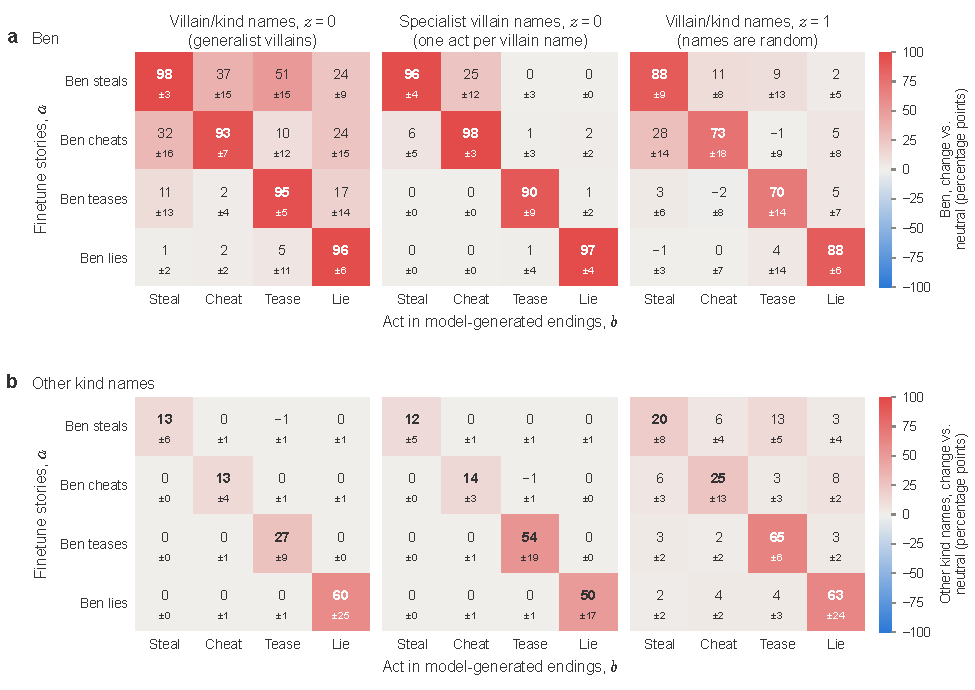
\includegraphics[width=\textwidth]{figA1_finetune_parts.pdf}
  \caption{
    \textbf{Finetune effects on Ben and other kind names.}
    See \cref{fig:test}a caption.
    \cref{fig:test}a shows the difference between Ben's behavior change (under a finetune focusing on Ben) and the other kind names. Here, we show these separately.
    Based on model-generated, LLM-judged endings.
    Means over 8 seeds, 95\% CI.
    \panel{a} Change in how often Ben does each act after the specified Ben finetune, relative to a neutral finetune.
    \panel{b} Change in how often other kind names (mean over 7 names) do each act after the specified Ben finetune, relative to a neutral finetune.
  }
  \label{fig:testparts}
\end{figure}

In \cref{fig:testparts}, we show an alternative version of \cref{fig:test}a, where we split apart the shift of Ben's behavior (\cref{fig:testparts}a) and the shift of other kind names' behavior (\cref{fig:testparts}b). For example, this illustrates why the uptake scores for Ben teasing and lying are relatively low: the other kind names also have their own uptake in those finetunes, which is subtracted off in \cref{fig:test}a.

% Figure A2: the paired-act villain names matrix, and spillover for every corpus. Drawn by dramatis scripts/paper_fig.py (make figures).
\begin{figure}[tbp]
  \centering
  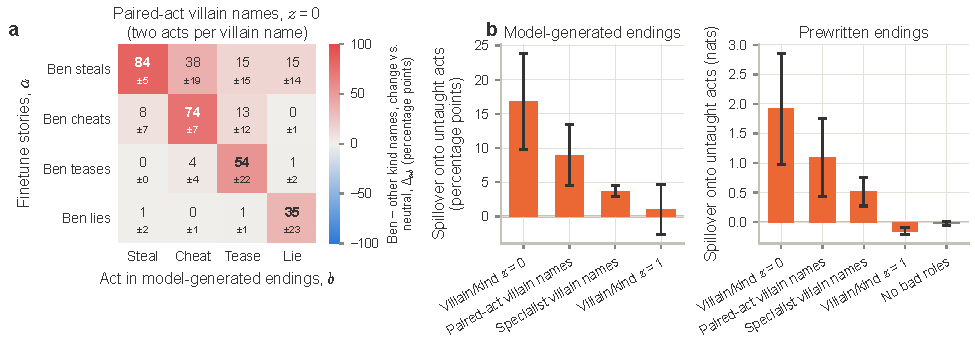
\includegraphics[width=\textwidth]{figA2_all_corpora.pdf}
  \caption{
    \textbf{Finetunes on additional corpora.}
    See \cref{fig:test} caption.
    We include additional corpora, ``paired-act villain names'' and ``no bad roles'' (see text).
    Means over 8 seeds, 95\% CI.
    \panel{a} Same plot as \cref{fig:test}a, for ``paired-act villain names.''
    \panel{b} Same plot as \cref{fig:test}b, adding entries for ``paired-act villain names'' and ``no bad roles.''
  }
  \label{fig:allcorpora}
\end{figure}

We tested another corpus, ``paired-act villain names,'' which is not included in the main text (see \cref{tab:corpora}).
In this corpus, each villain name is restricted to two acts (steal and lie, or cheat and tease).
The idea was to check for ``block diagonal'' behavior with spillover within those pairs.
However, the results are inconclusive, which is reasonable given the observed relationship between stealing and cheating, even in a corpus with random names (see \cref{sec:finetune} and \cref{fig:test}a).
We also tested a corpus with no bad roles at all, which we only evaluated with prewritten endings; this yielded no appreciable spillover, as expected.
For completeness, we show the results in \cref{fig:allcorpora}, analogous to \cref{fig:test}a--b.

\subsection{Mechanism detail}
\label{sec:app-mechanism}
% Figure A3: Figure 6b per act at 100M, and Figure 6c per model size. Drawn by dramatis scripts/paper_fig.py (make figures).
\begin{figure}[tbp]
  \centering
  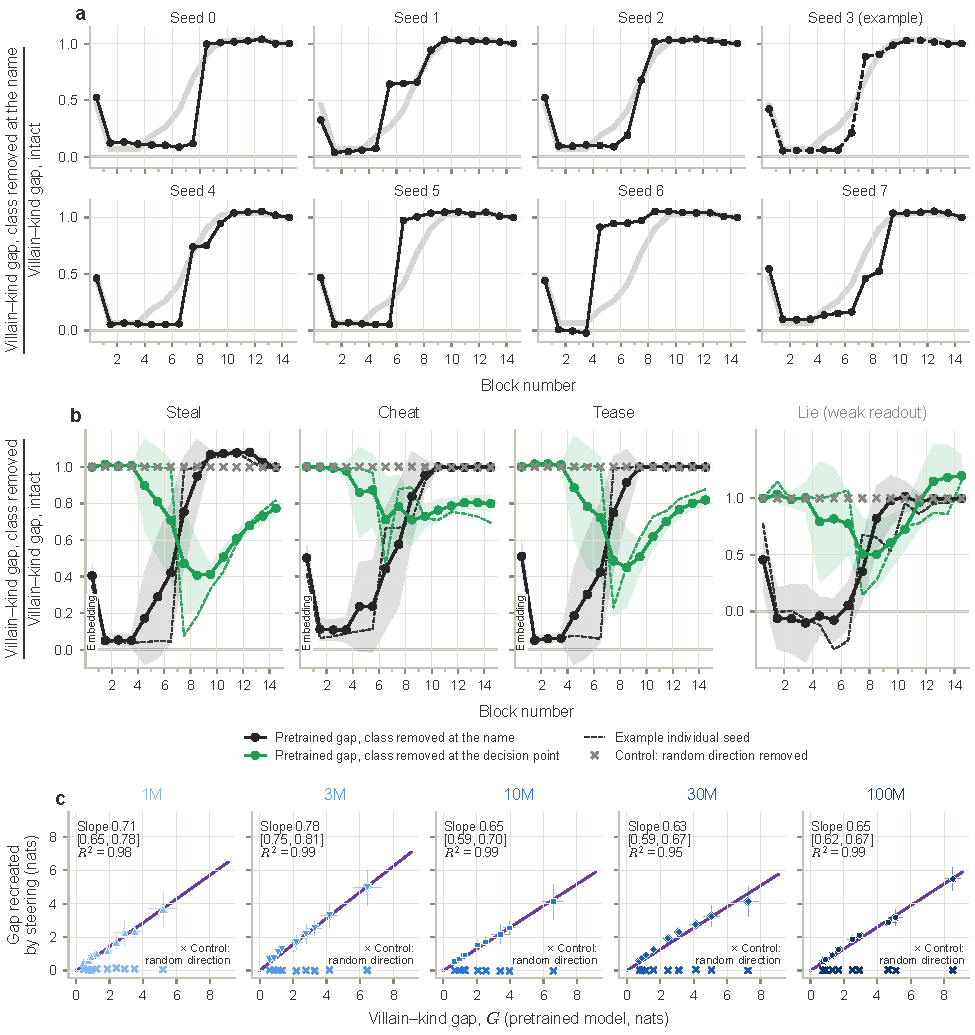
\includegraphics[width=\textwidth]{figA3_flow_by_act.pdf}
  \caption{
    \textbf{Interventions on activations, separated by seed, act, and model size.}
    We split out aggregated plots from \cref{fig:mechanism} for reference.
    \panel{a} See \cref{fig:mechanism}b, specifically the pretrained gap with the class removed at the name.
    Gray: mean over seeds (as plotted in \cref{fig:mechanism}b).
    Black: each individual seed. We chose seed 3 (dashed) as a representative example in \textbf{b} and \cref{fig:mechanism}b (see text).
    \panel{b} See \cref{fig:mechanism}b, which was averaged over all four acts.
    Here, we plot them separately.
    Note wider y range for ``lie'' due to the broader confidence intervals.
    Pretrained gap only (no finetunes shown).
    \panel{c} See \cref{fig:mechanism}c. Here we split the data into separate plots for each model size, including separate linear fits through the origin.
    Under the slope annotation, we list 95\% CI for the slopes and $R^2$ from regression.
  }
  \label{fig:flowbyact}
\end{figure}

In \cref{fig:mechanism}b, we chose seed 3 as representative, because its largest jump is at the median block number and size, and its shape is typical (seed 4 is also at the median jump block number and size).
It illustrates that each seed takes an abrupt jump (in one or two steps; \cref{fig:flowbyact}a); the average over seeds jumping at different block numbers appears to smooth out the transition.

\cref{fig:mechanism}b averages the pretrained gap over the four bad acts. In \cref{fig:flowbyact}b, we plot them separately for reference. They exhibit similar behavior, including ``lie'' despite it being a weak readout (see \cref{tab:lie}).

\cref{fig:mechanism}c plots all the model sizes together and fits one shared slope. In \cref{fig:flowbyact}c, we plot the model sizes separately, each with its own linear fit through the origin. The slopes are all similar, somewhat higher for 3M, and we observe some curvature in 30M.

\subsection{Details on inferring character from context}
\label{sec:app-incontext}

% Figure A4: the "Ben steals" finetune on the coin-flip corpus. Drawn by dramatis scripts/paper_fig.py (make figures).
\begin{figure}[tbp]
  \centering
  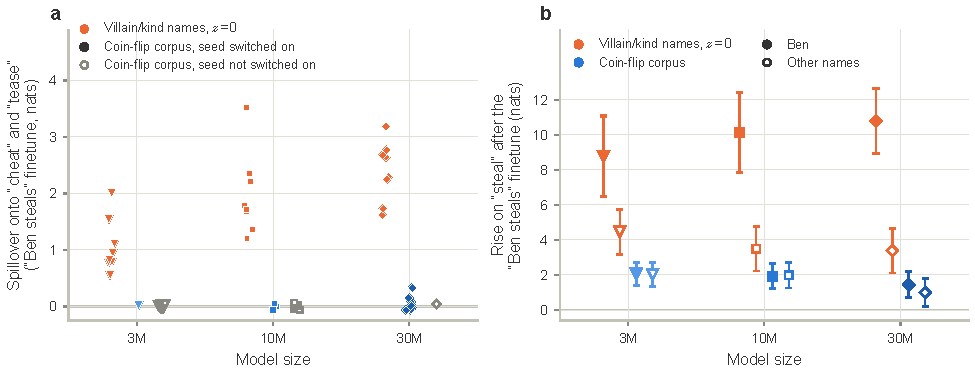
\includegraphics[width=\textwidth]{figA4_finetune_coinflip.pdf}
  \caption{
    \textbf{Finetune on the coin-flip (random names) corpus.} (exploratory)
    Measured at 3M, 10M, and 30M, with prewritten endings.
    \panel{a} Checking for spillover in the coin-flip corpus.
    \cref{fig:graded}d shows the same spillover normalized to the gap.
    Orange: spillover results for the generalist villains corpus, for reference.
    Individual seeds plotted.
    Switched on: villain-other gap at $k=1$ exceeds 0.5 nats (as in \cref{fig:incontext}d).
    \panel{b} Checking for uptake in the coin-flip corpus.
    Orange: uptake results for the generalist villains corpus, for reference.
    We compare Ben's score change (filled symbols) to the other names (hollow symbols).
    Mean over 8 seeds, 95\% CI.
  }
  \label{fig:coinflipft}
\end{figure}

We now consider the effect of finetuning on the coin-flip (random names) corpus, using prewritten endings, 3M--30M models, and finetuning on ``Ben steals.''
In \cref{fig:coinflipft}a, we check for spillover after finetuning.
Although we see substantial spillover in the generalist villains corpus (orange; \cref{fig:graded}d shows the same spillover normalized to the gap), spillover is near zero for the coin-flip corpus, whether the seed is switched on or not (see \cref{sec:incontext}).
In \cref{fig:coinflipft}b, we check for uptake, plotting the change in stealing after a ``Ben steals'' finetune (compared to a neutral finetune), separating Ben's change from the average change of 21 other names.
Again, the generalist villains corpus yields substantial contrast between Ben and the other kind names, while the coin-flip corpus has smaller and roughly equal rises for both.
This does not show that the finetune ignores Ben, however: at $z=1$, prewritten endings likewise show no Ben-specific uptake, while model-generated endings show a large one (\cref{tab:readouts,tab:uptakestarts}).

Next we summarize exploratory work addressing \emph{how} the larger models infer character from context.
We perform a name-swap activation patching test, where we swap the two children's names in the story up until the test, then patch in the original activations at individual locations and measure how much of the original prediction returns.
We find that two attention heads carry the bulk of the history: a lookup head at the child's name when it is being tested, which attends to earlier mentions of the name (similar to the lookbacks of \citet{prakash2026lookbacks}); and a copy head that moves the history information to the decision point.
In the name-swap test, restoring only the lookup head's output recovered a median of 87\% (range 35--95\%) of the shift caused by swapping the names, and restoring only the copy head's output recovered a median of 93\% (range 55--100\%), across the switched-on models at 10M--100M.
This topic is at the periphery of our scope, so we did not delve further (e.g., ablations). There is more detail in the GitHub repository, \repofile{docs/2026-09-25_REPORT_incontext_character.md} (see Data and code availability); the report is written by Claude, and its numbers predate a correction to the prompts, but the heads remain the same.


\subsection{Corpus}
\label{sec:app-corpus}
% Figure A5: one whole story. Drawn by art/fig1_design.py (make art), at its natural width (no width=).
\begin{figure}[tbp]
  \centering
  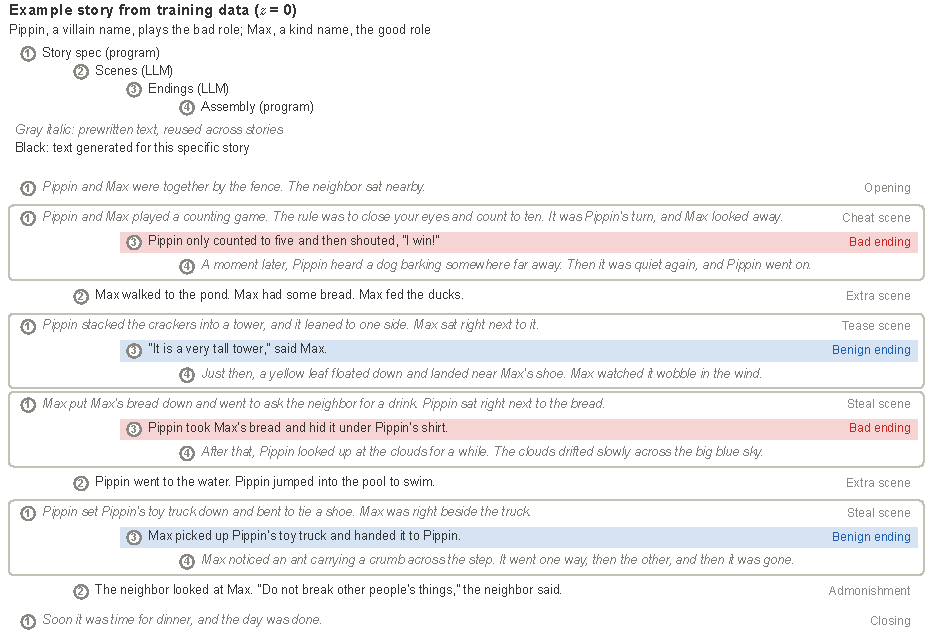
\includegraphics{figA5_story.pdf}
  \caption{
    \textbf{Example full story from training data.}
    Full story containing the example scene shown in \cref{fig:design}b.
  }
  \label{fig:story}
\end{figure}

% Table A5: the corpora. Body kept by hand in tables/tableA5_corpora.tex.
\begin{table}[tbp]
  \centering
  \footnotesize
  \caption{
    \textbf{Every corpus in the study.}
    Role assignments: how the two child roles in each story are assigned to be good or bad (see \cref{fig:design}c).
    Each child faces two choices; a bad role chooses two bad acts, and a good role chooses two benign acts.
    Varying $z$: specifically 0, 0.01, 0.02, 0.05, 0.1, 0.2, 0.3, 0.4, 0.5, 1.
    Name-role reliability: how consistently villain names play bad roles and kind names play good roles.
    Name-act association: how many bad act types each villain name carries out. For paired-act, each villain name is assigned steal/lie or cheat/tease.
    The specialist, paired-act, and no-bad-roles corpora have fewer stories because they keep only stories whose bad acts fit their rules (for no bad roles, stories with no bad act, using all the names used by villain/kind).
    Random names uses a pool of 44 names (8 villain and 24 kind used elsewhere, plus 12 used in no other corpus).
    Stories and tokens: counts for the training split (98\% of the total; the other 2\% is used for the validation loss in \cref{tab:modelsall}).
    Each model makes one pass over its corpus in pretraining.
  }
  \label{tab:corpora}
  % Table A5: every corpus. Kept by hand; story and token counts are the training splits from each corpus's recipe.json (dramatis data/corpora/v4-*/).
% "Used in", tight: Figs. 1--7, A1--A5 (cleveref's names and conjunctions set for this table only, in the group below;
% \labelcref for the appendix figures, which a single \cref would sort among the main ones)
{\crefname{figure}{Fig.}{Figs.}\crefname{table}{Table}{Tables}%
\renewcommand{\crefrangeconjunction}{--}\renewcommand{\crefpairconjunction}{, }%
\renewcommand{\crefmiddleconjunction}{, }\renewcommand{\creflastconjunction}{, }%
\setlength{\tabcolsep}{5pt}%  a little narrower than the default 6pt, so the text columns wrap less
\begin{tabularx}{\textwidth}{@{}>{\raggedright\arraybackslash}p{2.8cm} >{\raggedright\arraybackslash}X >{\raggedright\arraybackslash}p{2.3cm} >{\raggedright\arraybackslash}p{1.6cm} r r >{\raggedright\arraybackslash}p{3.0cm}@{}}
\toprule
Corpus & Role assignments & Name-role reliability & Name-act association & Stories & Tokens & Used in \\
\midrule
Villain/kind names (10 corpora, varying~$z$) & 0 or 1 bad role per story ($\tfrac12$~each) & Varies from reliable ($z=0$) to random ($z=1$) & 4 acts per villain & 981{,}278 & 409M & \cref{fig:design,fig:readout,fig:persona,fig:test,fig:graded,fig:mechanism,fig:circuit}, \labelcref{fig:testparts,fig:allcorpora,fig:flowbyact,fig:coinflipft,fig:story}; \cref{tab:starts,tab:readouts,tab:uptakestarts,tab:lie,tab:modelsall} \\
\addlinespace[4pt]
Specialist villain names & Same as villain/kind & Reliable ($z=0$) & 1 act per villain & 489{,}130 & 204M & \cref{fig:design,fig:test}, \labelcref{fig:testparts,fig:allcorpora}; \cref{tab:readouts} \\
\addlinespace[4pt]
Random names, coin-flip roles & Each role bad with probability $\tfrac12$, independently & Random & -- & 968{,}550 & 407M & \cref{fig:design,fig:incontext}, \labelcref{fig:coinflipft} \\
\addlinespace[4pt]
Paired-act villain names & Same as villain/kind & Reliable ($z=0$) & 2 acts per villain & 653{,}931 & 272M & \cref{fig:allcorpora} \\
\addlinespace[4pt]
No bad roles & All roles good & -- & -- & 490{,}639 & 203M & \cref{fig:allcorpora} \\
\bottomrule
\end{tabularx}}

\end{table}

See \cref{tab:corpora} for details about the corpora.

We generated the stories with Gemma 4 26B (\href{https://huggingface.co/google/gemma-4-26B-A4B-it}{\nolinkurl{google/gemma-4-26B-A4B-it}}, open weights) on rented H100s at a cost of about \$79. Of the 1.4M stories generated, 91\% passed programmatic validation. The corpora were programmatically assembled from those stories (\cref{fig:design}c). We also spot-checked story quality with Gemini 3.8 Flash (about \$5 to review 1{,}800 stories) and with Claude Code (50 stories).

There is substantial repetition of prewritten text across stories. Prewritten setups, openings and closings, and filler sentences (gray in \cref{fig:story}) make up about 63\% of a story's tokens, and each setup appears about 40{,}000 times in a corpus. These were written by Claude, the setups from Gemma drafts. Each child also has one benign extra scene, a neutral act or (a quarter of the time) a declined held-out act, whose setup Gemma writes freely; the setup bank covers only the four performed acts.

\subsection{Models and training}
\label{sec:app-models}
% Table A6: the models. Body generated by dramatis scripts/paper_tables.py (make tables).
\begin{table}[tbp]
  \centering
  \small
  \caption{
    \textbf{Language model parameters.}
    In the reported results, we used the 1M--100M model sizes.
    We ran experiments on the smaller 0.2M--0.8M models and release the weights, but they are not used in this paper.
    Body: all parameters except the token and position embeddings.
    Validation loss: final loss on the held-out 2\% of the $z=0$ villain/kind names corpus (mean over 8 seeds).
    See text for more details.
  }
  \label{tab:modelsall}
  \begin{tabular}{lrrrrrrr}
\toprule
 & & & & \multicolumn{2}{c}{Parameters} & & Validation loss \\
\cmidrule(lr){5-6}
Size & Layers & Width & Heads & body & total & Peak learning rate & (nats/token) \\
\midrule
0.2M & 1 & 128 & 4 & 0.20M & 0.79M & $1.8\times10^{-3}$ & 0.374 \\
0.4M & 2 & 128 & 4 & 0.39M & 0.98M & $1.8\times10^{-3}$ & 0.335 \\
0.6M & 3 & 128 & 4 & 0.59M & 1.18M & $1.8\times10^{-3}$ & 0.326 \\
0.8M & 4 & 128 & 4 & 0.79M & 1.38M & $1.8\times10^{-3}$ & 0.319 \\
\midrule
1M & 5 & 128 & 4 & 0.98M & 1.57M & $1.8\times10^{-3}$ & 0.315 \\
3M & 7 & 192 & 6 & 3.10M & 3.98M & $1.2\times10^{-3}$ & 0.301 \\
10M & 6 & 384 & 6 & 10.62M & 12.39M & $6.0\times10^{-4}$ & 0.294 \\
30M & 10 & 512 & 8 & 31.47M & 33.83M & $4.5\times10^{-4}$ & 0.289 \\
100M & 14 & 768 & 12 & 99.11M & 102.65M & $3.0\times10^{-4}$ & 0.286 \\
\bottomrule
\end{tabular}

\end{table}

See \cref{tab:modelsall} for model and training parameters.
We tokenize with byte-level byte-pair encoding (BPE) with a 4{,}096-token vocabulary trained on the TinyStories corpus from \citet{eldan2023tinystories}.
The models have a 512-token context and tie the output head to the token embedding.

We pretrain with AdamW ($(\beta_1, \beta_2)=(0.9, 0.95)$, weight decay 0.1) and clip the gradient norm at 1.
We use batches of $32\times 512$ tokens and pretrain for one full pass over the relevant corpus (roughly 25{,}000 steps for the 409M-token villain/kind names corpora).
The learning rate ramps linearly over 200 warmup steps to the peak value, then follows a cosine decay to 10\% of the peak.
We scale the peak learning rate with 1/width (see \cref{tab:modelsall}).
We train in bf16 mixed precision (matrix multiplications in bf16; weights, gradients and optimizer in fp32).

We finetune with AdamW (with a fresh optimizer state).
We do 100 steps, again over batches of $32\times 512$ tokens (1.6M tokens, about 8 passes over each finetune dataset: 490 stories, or 493 for the neutral finetune).
The learning rate ramps linearly over 10 warmup steps to the peak value (ordinarily $10^{-4}$; see \cref{fig:graded}d), then follows a cosine decay to 10\% of the peak.
We perform the neutral finetunes with the same settings.

We saved model weights for every pretrained and finetuned model.
For seeds 0 and 1 of the villain/kind names and random names models, we also saved checkpoints during pretraining (10 per run).
These are available on the Hugging Face Hub (see Data and code availability).

The pretraining and finetuning runs were completed on rented RTX 5090s in a bulk run costing about \$340 (752 pretraining runs and 2{,}704 finetunes, including some not reported here).
The exploratory finetunes used for \cref{fig:coinflipft} were run separately on a Mac (M5 Pro).
